\documentclass[CJKutf8,dvipsnames,table]{beamer}
\usepackage{hyperref}
\hypersetup{
  pdftitle={Signals and Systems},
  pdfauthor={Hong MingJian},
  pdfsubject={Introduction},
  pdfpagemode={FullScreen},
  colorlinks={true},
  linkcolor={blue},
}

%% https://tex.stackexchange.com/questions/47576/combining-ifxetex-and-ifluatex-with-the-logical-or-operation
\usepackage{ifxetex,ifluatex}
\newif\ifxetexorluatex % a new conditional starts as false
\ifnum 0\ifxetex 1\fi\ifluatex 1\fi>0
   \xetexorluatextrue
\fi
\usepackage{ifplatform}
\ifxetexorluatex
	\usepackage[slantfont,boldfont]{xeCJK}
	\ifwindows
		\setCJKmainfont{SimSun} % Windows默认中文字体:中易宋体
	\fi
	\ifmacosx
		\setCJKmainfont{STSong} % MacOS默认中文字体:华文宋体
	\fi
	\iflinux
		\setCJKmainfont{Noto Serif CJK SC} % Linux默认中文字体:思源宋体(By Adobe & Google)
	\fi
\else
	\usepackage{CJKutf8}
\fi

\usepackage[export]{adjustbox}
\usepackage{mathptmx} %pdfTeX error: pdflatex (file fmex9.pfb): cannot open Type 1 font file for reading
                                                 %https://forum.ubuntu.com.cn/viewtopic.php?t=269943
\usepackage{mathtools}
\usepackage[mathscr]{urwchancal}

\usetheme{Madrid}%{Warsaw}
\usecolortheme{default}

%gets rid of bottom navigation bars
\setbeamertemplate{footline}[page number]{}
%gets rid of navigation symbols
\setbeamertemplate{navigation symbols}{}

\begin{document}
\ifxetexorluatex\else
\begin{CJK*}{UTF8}{song}
\fi

  \title{数字信号处理}
  \subtitle{第7讲:离散傅立叶变换}
  \author{洪明坚}
  \institute{重庆大学软件学院}
  \date{\today}

  \AtBeginSection[]
  {
    \begin{frame}
      \frametitle{Outline}
      \tableofcontents[currentsection]
    \end{frame}
  }

  \frame{\titlepage}
  \frame{\frametitle{目录}\tableofcontents}
  
  \section{离散傅里变换}
  
    %% PAGE
  \begin{frame}
    \frametitle{引入}
    \begin{itemize}
    \item 实际问题中处理的信号,一般都有有限长度。
    	\begin{itemize}
    	\item 将一段有限长的时域序列信号,变换为对应的有限长的频域序列,反之亦然。
		\item 以方便计算机或数字电路实现
    	\end{itemize}
	\item 因此,需要一种在时域和频域都是离散的、且有限长的变换
		\begin{itemize}
		\item 离散傅立叶变换(Discrete Fourier Transform, DFT)是其中最重要的变换。
		\end{itemize}
    \end{itemize}
  \end{frame} 

  %% PAGE
  \begin{frame}
    \frametitle{引入}
    \begin{itemize}
    \item 设$x[n]$是一个有限长信号,即存在一个整数$N_1$,在$0\leq n \leq N_1 - 1$外有$x[n]=0$。
    	\begin{itemize}
    	\item $x[n]$的傅立叶变换为$X(e^{j\omega})$
    	\end{itemize}
	\item 取$N\geq N_1$,构造一个周期为$N$的信号$\tilde{x}[n]$,使得$\tilde{x}[n]$在一个周期内等于$x[n]$,即以N为周期进行延拓
		\[
			\tilde{x}[n]=\sum_{r=-\infty}^{\infty} x[n+rN]
		\]
		\begin{itemize}
		\item 为简洁起见,记
		\[
			\tilde{x}[n]=x[((n))_N]
		\]
		\end{itemize}
	\item 则$\tilde{x}[n]$的傅立叶级数系数
		\begin{align*}
			\tilde{X}[k] & = \frac{1}{N}\sum_{n=<N>} \tilde{x}[n] e^{-jk(2\pi/N)n} \\
		    	& = \frac{1}{N}\sum_{n=0}^{N-1} x[n] e^{-jk(2\pi/N)n}, k \in \mathbb{Z}
		\end{align*}
		\begin{itemize}
		\item $\tilde{X}[k]=\tilde{X}[k+N]$
		\end{itemize}
    \end{itemize}
  \end{frame} 	

  %% PAGE
  \begin{frame}
    \frametitle{DFT}
    \begin{itemize}
	\item 长度为$N_1$的信号$x[n]$的$N$点DFT,$N \geq N_1$
		\[
			X[k] = \frac{1}{N}\sum_{n=0}^{N-1} x[n] e^{-jk(2\pi/N)n}, k=0, 1, \hdots, N-1
		\]
		\begin{itemize}
		\item 显然,$\tilde{X}[k]=X[((k))_N]$
		\end{itemize}
	{\color{red}即$x[n]$的N点DFT,是$\tilde{x}[n]$的DTFS系数$\tilde{X}[k]$的一个周期}
	\item 可以从$X[k]$中恢复$x[n]$,即离散傅立叶逆变换(IDFT)
		\[
			x[n] = \sum_{k=0}^{N-1} X[k] e^{jk(2\pi/N)n}, n=0, 1, \hdots, N-1
		\]
	\item 记为
		\[
			x[n] \xleftrightarrow{\mathscr{DFT}} X[k]
		\]		
    \end{itemize}
  \end{frame} 	
	
  %% PAGE
  \begin{frame}
    \frametitle{DFT:矩阵表示}
    \begin{itemize}
	\item 记
	\begin{align*}
		%W_N & = e^{-j(2\pi/N)} \\
		\mathbf{x} & =[x[0], x[1], \hdots, x[N-1]]^T \\
		\mathbf{X} & =[X[0], X[1], \hdots, X[N-1]]^T
	\end{align*}
	\[
	\mathbf{D}_N=
    \begin{pmatrix}
1      & 1   & 1     & ... & 1 \\
1      & W_N & W_N^2 & ... & W_N^{N-1} \\
1      & W_N^2 & W_N^4 & ... & W_N^{2(N-1)} \\
\vdots & \vdots & \vdots  & \ddots & \vdots \\
1      & W_N^{N-2} & W_N^{2(N-2)} & ... & W_N^{(N-1)(N-2)} \\
1      & W_N^{N-1} & W_N^{2(N-1)} & ... & W_N^{(N-1)^2} \\

	\end{pmatrix}
	, W_N  = e^{-j(2\pi/N)}
	\]	
	\end{itemize}
  \end{frame} 	
  	
  %% PAGE
  \begin{frame}
    \frametitle{DFT:矩阵表示}
    \begin{itemize}
	\item DFT
	\[
		\mathbf{X}=\mathbf{D}_N \mathbf{x}
	\]
	\item IDFT
	\[
		\mathbf{x}=\mathbf{D}_N^{-1} \mathbf{X}
	\]
	且
	\[
		\mathbf{D}_N^{-1}=\frac{1}{N}\mathbf{D}_N^{*}
	\]
	\end{itemize}
  \end{frame} 
  	
  %% PAGE
  \begin{frame}
    \frametitle{Questions}
    \begin{itemize}
    \item Any questions?
    \end{itemize}
    \begin{center}
      
\includegraphics[scale=.5]{question}
    \end{center}
  \end{frame} 

  %% PAGE
  \begin{frame}
    \frametitle{例子}
    \begin{itemize}
	\item 计算如下$x[n]$的5点DFT
		\begin{center}
      	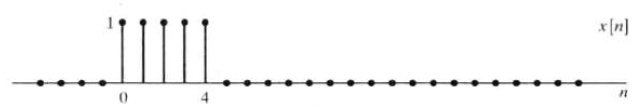
\includegraphics[scale=.25]{dtsp-c-f8-10a}
    	\end{center}
	\item 构造$\tilde{x}[n]$如下
		\begin{center}
      	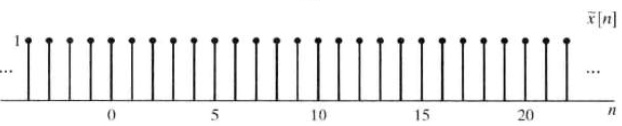
\includegraphics[scale=.25]{dtsp-c-f8-10b}
    	\end{center}	
	\item 则
	\[
\tilde{X}[k] = \sum_{n=0}^{4} e^{-j(2\pi k/5)n} = 
\left\{
    \begin {aligned}
         & 5 \quad & k = 0, \pm5, \pm 10, \hdots \\
         & 0 \quad & otherwise
    \end{aligned}
\right.			
	\]
		\begin{center}
      	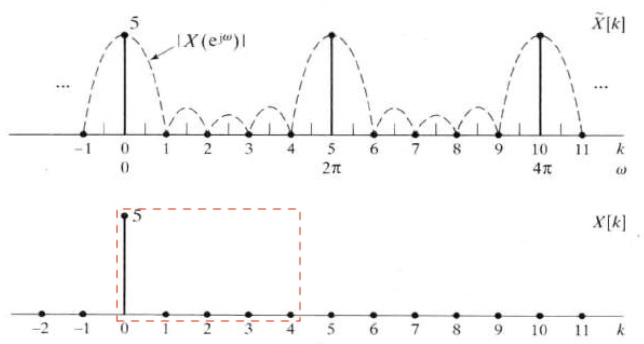
\includegraphics[scale=.28]{dtsp-c-f8-10cd}
    	\end{center}	
	\end{itemize}
  \end{frame}   
  
  %% PAGE
  \begin{frame}
    \frametitle{例子}
    \begin{itemize}
	\item 10点DFT
		\begin{center}
      	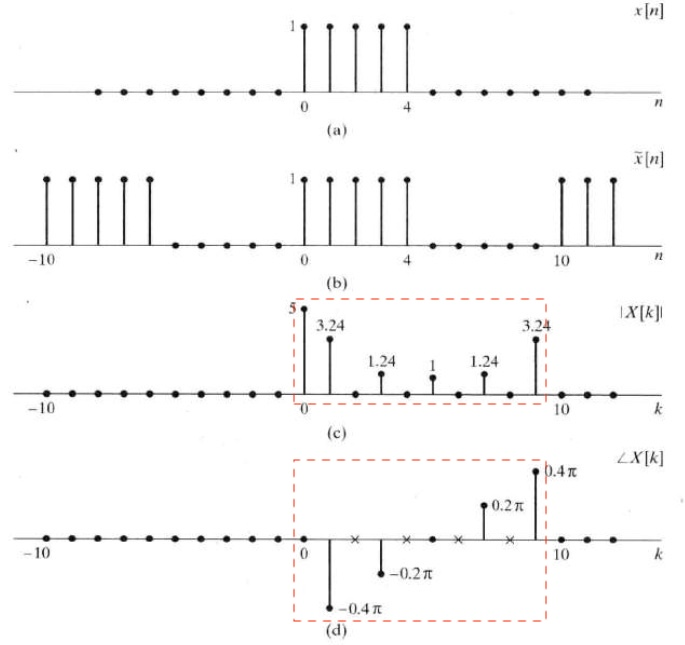
\includegraphics[scale=.35]{dtsp-c-f8-11}
    	\end{center}	
	\end{itemize}
  \end{frame}  

  %% PAGE
  \begin{frame}
    \frametitle{与DTFT的关系}
    \begin{itemize}
	\item 根据DTFT的定义,长度为N的序列$x[n]$的傅立叶变换
	\[
		X(e^{j\omega}) = \sum_{n=-\infty}^{\infty}x[n]e^{-j\omega n} =  \sum_{n=0}^{N-1}x[n]e^{-j\omega n} 	
	\]
	$X(e^{j\omega})$以$2\pi$为周期
	\item 对一个周期内的$X(e^{j\omega})$进行等间隔采样,即
	\[
	\left. X(e^{j\omega}) \right\rvert_{\omega=2\pi k/N}	 = \sum_{n=0}^{N-1}x[n]e^{-jk(2\pi /N) n} = X[k], k=0, 1, \hdots, N-1
	\]	
	也就是说,{\color{red}$x[n]$的$N$点DFT是对一个周期内的$X(e^{j\omega})$以等间隔$2\pi/N$采样的结果}

	\end{itemize}
  \end{frame}      
    
  %% PAGE
  \begin{frame}
    \frametitle{Questions}
    \begin{itemize}
    \item Any questions?
    \end{itemize}
    \begin{center}
      
\includegraphics[scale=.5]{question}
    \end{center}
  \end{frame}   
  
	\section{离散傅里变换的性质}
	
  %% PAGE
  \begin{frame}
    \frametitle{性质}
    \begin{itemize}
    \item 线性:若$x_1[n] \xleftrightarrow{\mathscr{DFT}} X_1[k]$, $x_2[n] \xleftrightarrow{\mathscr{DFT}} X_2[k]$,则
    \[
    ax_1[n]+bx_2[n] \xleftrightarrow{\mathscr{DFT}} aX_1[k]+bX_2[k]
    \]
    注意:若$x_1[n]$的长度是$N_1$,且$x_2[n]$的长度是$N_2$,要以$N \geq max(N_1, N_2)$点计算$x_1[n]$和$x_2[n]$的DFT。

	\end{itemize}
  \end{frame}  
      
  %% PAGE
  \begin{frame}
    \frametitle{性质}
    \begin{itemize}
    \item 循环位移
    \[
    	x[((n-m))_N], 0 \leq n \leq N-1 \xleftrightarrow{\mathscr{DFT}} e^{-j(2\pi k/N)m}X[k]=W_N^m X[k]
    \]
        \begin{center}
      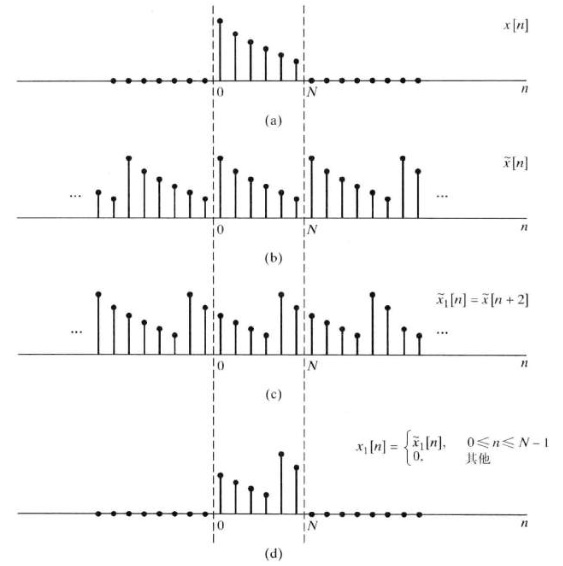
\includegraphics[scale=.35]{dtsp-c-f8-12}
    \end{center}
	\end{itemize}
  \end{frame}        
      
  %% PAGE
  \begin{frame}
    \frametitle{性质}
    \begin{itemize}
    \item 循环卷积(Circular convolution):若$x_1[n]$和$x_2[n]$的长度分别是$N_1$和$N_2$,定义$N$点循环卷积
    \[
    	x_1[n] \textcircled{N} x_2[n]=\sum_{m=0}^{N-1}x_1[m]x_2[((n-m))_N], 0 \leq n \leq N-1
    \]
    其中$N\geq max(N_1, N_2)$。则
    \[
		x_1[n] \textcircled{N} x_2[n] \xleftrightarrow{\mathscr{DFT}} X_1[k]X_2[k]
	\]    
	根据对偶性质,反过来也成立
	\[
		x_1[n]x_2[n] \xleftrightarrow{\mathscr{DFT}} \frac{1}{N} X_1[k] \textcircled{N} X_2[k]
	\] 
	\end{itemize}
  \end{frame}         
      
  %% PAGE
  \begin{frame}
    \frametitle{性质}
    \begin{itemize}
    \item 汇总
  		\begin{center}
   		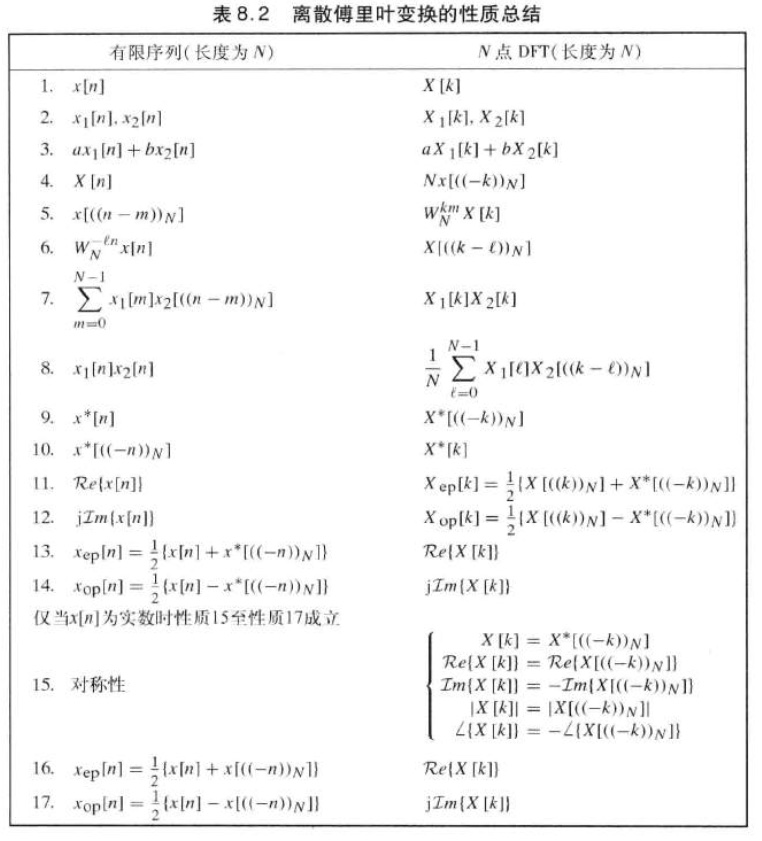
\includegraphics[scale=.27]{dtsp-c-t8-2}
   		\end{center}    
	\end{itemize}
  \end{frame} 
        
  %% PAGE
  \begin{frame}
    \frametitle{Questions}
    \begin{itemize}
    \item Any questions?
    \end{itemize}
    \begin{center}
      
\includegraphics[scale=.5]{question}
    \end{center}
  \end{frame}  
        
  \section{循环卷积}
  
  %% PAGE
  \begin{frame}
    \frametitle{循环卷积}
    \begin{itemize}
    \item $x_1[n]$和$x_2[n]$的$N$点循环卷积
    \[
    	x_1[n] \textcircled{N} x_2[n]=\sum_{m=0}^{N-1}x_1[m]x_2[((n-m))_N], 0 \leq n \leq N-1
    \]    
    \item 具体计算
    	\begin{itemize}
		\item 令$n=0$,当$m=0, 1, \hdots, N-1$时
		\begin{align*}
			\{ x_2[((0))_N], x_2[((-1))_N], x_2[((-2))_N], \hdots, x_2[((-N+1))_N] \} & \\
		  = \{ x_2[0], x_2[N-1], x_2[N-2], \hdots, x_2[1] \} & 
		\end{align*}
		
		\item 令$n=1$,当$m=0, 1, \hdots, N-1$时
		\begin{align*}
			\{ x_2[((1))_N], x_2[((0))_N], x_2[((-1))_N], \hdots, x_2[((-N+2))_N] \} & \\
		  = \{ x_2[1], x_2[0], x_2[N-1], \hdots, x_2[2] \} & 
		\end{align*}	
		
		\item 以此类推	
		\end{itemize} 
	\end{itemize}
  \end{frame} 
        
  %% PAGE
  \begin{frame}
    \frametitle{循环卷积}
    \begin{itemize}
    \item $N$点循环卷积的右边可以写成矩阵形式
	\[
			%x_1[n] \textcircled{N} x_2[n] =
        \begin{pmatrix}
        x_2[0]      & x_2[N-1]   & x_2[N-2]  & ... & x_2[1] \\
        x_2[1]      & x_2[0]     & x_2[N-1]  & ... & x_2[2] \\
        x_2[2]      & x_2[1]     & x_2[0]    & ... & x_2[3] \\
        \vdots & \vdots & \vdots & \ddots & \vdots           \\
        x_2[N-2]    & x_2[N-3]   & x_2[N-4]  & ... & x_2[N-1] \\
        x_2[N-1]    & x_2[N-2]   & x_2[N-3]  & ... & x_2[0] \\
        \end{pmatrix}	
        \begin{pmatrix}
        x_1[0]  \\
        x_1[1]  \\
        x_1[2]  \\
        ...     \\
        x_1[N-2] \\
        x_1[N-1]
        \end{pmatrix}
	\]
		   
	\end{itemize}
  \end{frame}  
        
  %% PAGE
  \begin{frame}
    \frametitle{循环卷积}
    \begin{itemize}
    \item 图示
   		\begin{center}
   		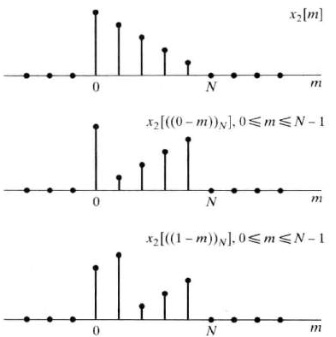
\includegraphics[scale=.6]{dtsp-c-f8-14acd}
   		\end{center}    
	\end{itemize}
  \end{frame} 

  %% PAGE
  \begin{frame}
    \frametitle{与线性卷积的关系}
    \begin{itemize}
    \item 根据定义
    \begin{align*}
	    x_L[n] = x_1[n] \ast x_2[n] & = \sum_{m=0}^{N_1-1}x_1[m]x_2[n-m], n \in \mathbb{Z}    \\ 	
	    x_C[n] = x_1[n] \textcircled{N} x_2[n] & = \sum_{m=0}^{N-1}x_1[m]x_2[((n-m))_N], 0 \leq n \leq N-1 	    
    \end{align*}
    其中,
    \begin{align*}
	    N & \geq max(N_1, N_2) \\
	    x_2[((n))_N] & = \sum_{r=-\infty}^{\infty} x_2[n+rN]
	\end{align*}
	\end{itemize}
  \end{frame} 
  
  %% PAGE
  \begin{frame}
    \frametitle{与线性卷积的关系}
    \begin{itemize}
    \item 所以
    \begin{align*}
	    x_C[n] & = \sum_{m=0}^{N-1}x_1[m]x_2[((n-m))_N] 	\\    
	    & = \sum_{m=0}^{N-1}x_1[m]\sum_{r=-\infty}^{\infty} x_2[n-m+rN] \\
	    & = \sum_{r=-\infty}^{\infty} \sum_{m=0}^{N-1}x_1[m] x_2[n-m+rN], 0 \leq n \leq N-1 	    
    \end{align*}
    根据线性卷积的定义,
    \[
    \sum_{m=0}^{N-1}x_1[m] x_2[n-m+rN] = x_L[n+rN]
    \]
    所以
	\[
		x_C[n] = \sum_{r=-\infty}^{\infty} x_L[n+rN], 0 \leq n \leq N-1
	\]
	\end{itemize}
  \end{frame}   
  
  %% PAGE
  \begin{frame}
    \frametitle{与线性卷积的关系}
    \begin{itemize}
    \item 再写一遍公式
    \[
		x_C[n] = \sum_{r=-\infty}^{\infty} x_L[n+rN], 0 \leq n \leq N-1
	\]
    \item 也就是说,{\color{red} 把线性卷积$x_L[n]$以$N$为周期进行延拓,然后取$0, 1, 2, \hdots, N-1$共$N$个点,就是$N$点循环卷积。}
    	\begin{itemize}
    	\item 线性卷积$x_L[n]$的长度是$N_1+N_2-1$。所以
			\begin{itemize}
    		\item 如果$N < (N_1+N_2-1)$,那么$x_C[n]$将被相邻的$x_L[n]$混叠。
			\item 因此,{\color{red} 当$N \geq (N_1+N_2-1)$时,$N$点循环卷积等于线性卷积}
			\end{itemize}
    	\end{itemize}

	\end{itemize}
  \end{frame} 

  %% PAGE
  \begin{frame}
    \frametitle{与线性卷积的关系}
    \begin{itemize}
    \item 因为DFT有快速算法FFT(Fast Fourier Transform),用DFT计算线性卷积要比直接计算快
	\[
		y[n] = x_1[n] \ast x_2[n]
	\]
	取$N=N_1+N_2-1$
    \begin{center}
      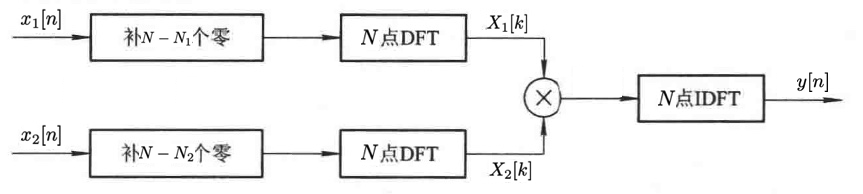
\includegraphics[scale=.37]{gxq-dsp-f3-4-1}
    \end{center}
	\end{itemize}
  \end{frame}   
  
  %% PAGE
  \begin{frame}
    \frametitle{Questions}
    \begin{itemize}
    \item Any questions?
    \end{itemize}
    \begin{center}
      
\includegraphics[scale=.5]{question}
    \end{center}
  \end{frame}  
  
  \section{2维离散傅立叶变换}

  %% PAGE
  \begin{frame}
    \frametitle{2-D DFT}
    \begin{itemize}
    \item $f[x, y]$是2维离散信号(如图像),大小为$M \times N$。\\
    DFT
    \[
    	F[u, v] = \sum_{x=0}^{M-1} \sum_{y=0}^{N-1} f[x, y] e^{-j2\pi (ux/M+vy/N)}
    \]
    IDFT
    \[
    	f[x, y] = \frac{1}{MN}\sum_{u=0}^{M-1} \sum_{v=0}^{N-1} F[u, v] e^{j2\pi (ux/M+vy/N)}    
    \]
    
    \item
    \[
    	F[u, v] = |F[u, v]|e^{j\phi[u, v]}
    \]
    称$|F[u, v]|$为幅度谱,$\phi[u,v]$为相位谱
    \[
    	\phi[u, v] = arctan\frac{\mathit{Im}\{F[u, v]\}}{\mathit{Re}\{F[u, v]\}}
    \]
    \end{itemize}
    
  \end{frame}  
  
    %% PAGE
  \begin{frame}
    \frametitle{性质}
    \begin{itemize}
    \item 旋转:用极坐标表示    
    \[
    	x=rcos\theta, y=rsin\theta, u = \omega cos\phi, v=\omega sin \phi
    \]
    则
    \[
    	f[r, \theta+\theta_0] \xleftrightarrow{\mathscr{DFT}} F[\omega, \phi+\theta_0]
    \]
    即时域(其实是空域)旋转$\theta_0$,频域也旋转相同的角度。
    \end{itemize}
  \end{frame}  
  
    %% PAGE
  \begin{frame}
    \frametitle{性质}
    \begin{itemize}
    \item 可分性(Separability)    
    \begin{align*}
    	F[u, v] & = \sum_{x=0}^{M-1} \sum_{y=0}^{N-1} f[x, y] e^{-j2\pi (ux/M+vy/N)} \\
	            & = \sum_{x=0}^{M-1} e^{-j2\pi ux/M} \sum_{y=0}^{N-1} f[x, y] e^{-j2\pi vy/N} \\
	            & = \sum_{x=0}^{M-1} e^{-j2\pi ux/M} F[x, v]
    \end{align*}
    其中
    \[
	    F[x, v] = \sum_{y=0}^{N-1} f[x, y] e^{-j2\pi vy/N}
    \]
    也就是说,{\color{red}2-D DFT可以通过1-D DFT计算:先逐行(列)做1-D DFT,然后再逐列(行)做1-D DFT}。    
    \end{itemize}
  \end{frame}  
    
  %% PAGE
  \begin{frame}
    \frametitle{Questions}
    \begin{itemize}
    \item Any questions?
    \end{itemize}
    \begin{center}
      
\includegraphics[scale=.5]{question}
    \end{center}
  \end{frame}  
  
\ifxetexorluatex\else
\end{CJK*}
\fi
\end{document}

%%% Local Variables: 
%%% mode: latex
%%% TeX-master: t
%%% End: 
